

\subsection{Serverová část komponenty}\label{subsec:serverováČást}

Serverová část je odpovědná za propagaci jednotlivých operací mezi klienty připojenými k dokumentu a jejich persistenci pro nově připojené budoucí klienty.
Struktura serverové části je znázorněna pomocí třídním diagramu na obrázku~\ref{fig:DocumentServer}.
Základem této části je třída \texttt{DocumentServer} (reimplementace třídy Server z knihovny OT.js) a v případě navrhovaného prototypu aplikace i její potomek \texttt{DocumentSocketIOServer}.

\begin{figure}[ht!]
    \centering
    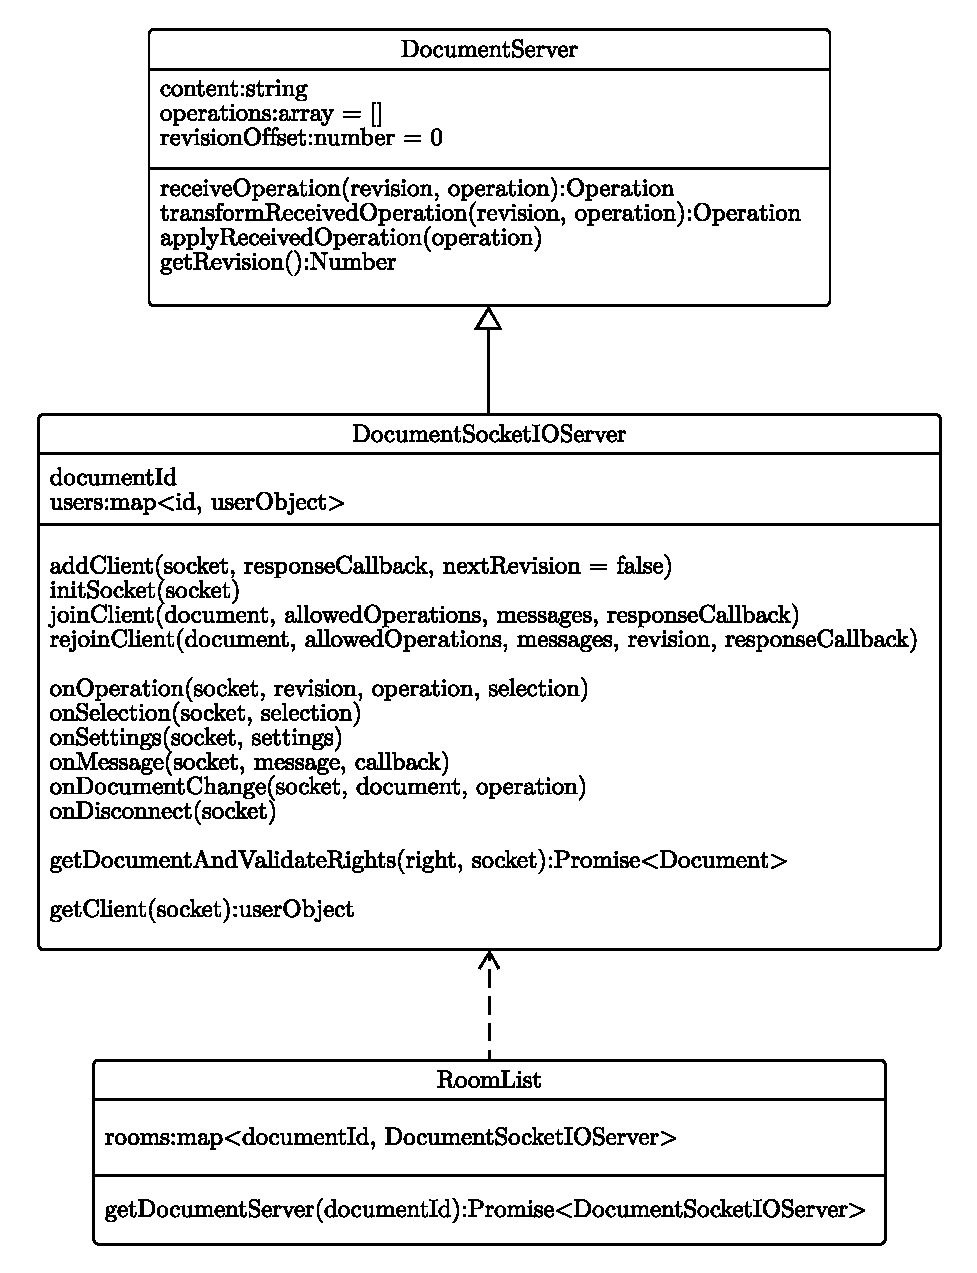
\includegraphics[width=.8\textwidth]{partials/navrh/editor/DocumentServer.pdf}
    \caption{Třídní diagram serverové části komponenty}\label{fig:DocumentServer}
\end{figure}

Instance třídy \texttt{DocumentServer} (respektive \texttt{DocumentSocketIOServer}) představuje jeden document a je zodpovědná o implementaci serverové části algoritmu~\gls{OT}.
Stará se o transformaci přijaté operace oproti souběžným, ale již schváleným operacím, a propaguje tuto transformovanou operaci ostatním uživatelům.

Další třídou, kterou je vhodné zmínit je třída \texttt{RoomList}, která udržuje informace o již existujících instancích třídy \texttt{DocumentSocketIOServer}, vytváří nové instance v případě, že pro daný dokument dosud neexistuje, a naslouchá novým socket.io spojení s klienty, které dále předává příslušným instancím třídy \texttt{DocumentServer}.
